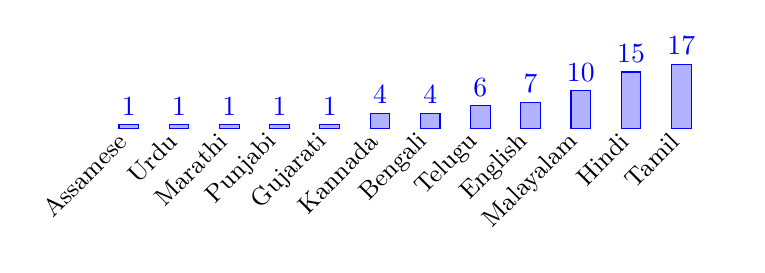
\begin{tikzpicture}
  \begin{axis}[
    ybar,
    width=10cm,
    height=2.5cm,
    ylabel={Count},
    symbolic x coords={
        Assamese,
        Urdu,
        Marathi,
        Punjabi,
        Gujarati,
        Kannada,
        Bengali,
        Telugu,
        English,
        Malayalam,
        Hindi,
        Tamil
    },
    xtick=data,
    nodes near coords,
    nodes near coords align={vertical},
    x axis line style = { opacity = 0 },
    axis y line       = none,
    tickwidth         = 0pt,
    enlarge x limits  = 0.1,
    bar width=0.25cm,
    ylabel style={font=\large, align=center, text=black},
    xlabel style={font=\large, align=center, text=black},
    xticklabel style={font=\small, text=black, rotate=45, anchor=east},
    yticklabel style={font=\small, text=black}
  ]
  \addplot coordinates {
    (Assamese,1)
    (Urdu,1)
    (Marathi,1)
    (Punjabi,1)
    (Gujarati,1)
    (Kannada,4)
    (Bengali,4)
    (Telugu,6)
    (English,7)
    (Malayalam,10)
    (Hindi,15)
    (Tamil,17)
  };
  \end{axis}
\end{tikzpicture}

